\documentclass[border=10pt]{standalone}
\usepackage{xcolor}
\usepackage{pgfplots}
\usepackage{tikz}
\begin{document}
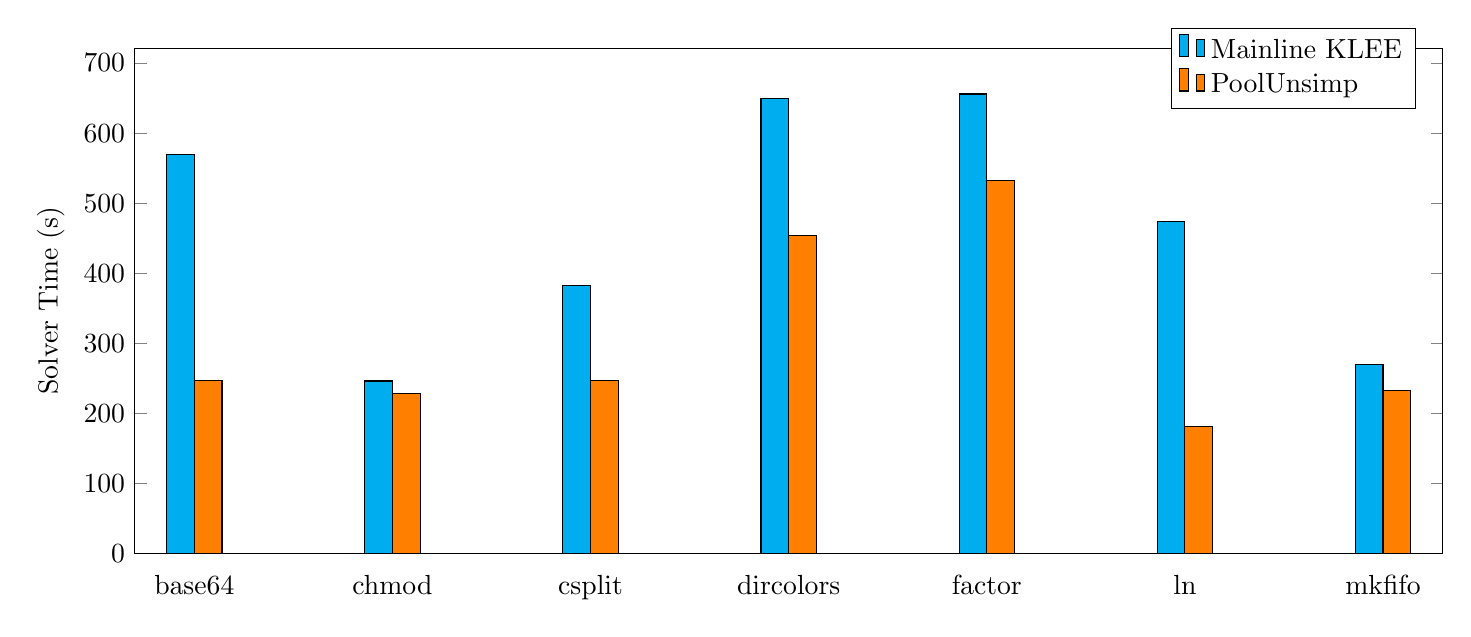
\begin{tikzpicture}
    \begin{axis}[
        width  = 1.5 * \textwidth,
        height = 8cm,
        major x tick style = transparent,
        % tickwidth=10,
        ybar=0,
        bar width=10pt,
        % ymajorgrids = true,
        ylabel = {Solver Time (s)},
        symbolic x coords={base64,chmod,csplit,dircolors,factor,ln,mkfifo},
        xtick = data,
        scaled y ticks = false,
        enlarge x limits=0.05,
        ymin=0,
        legend cell align=left,
        legend style={
                at={(0.98,0.88)},
                anchor=south east,
                % column sep=1ex
        }
    ]
        \addplot[style={cyan,fill=cyan,mark=none}, draw=black]
	coordinates {(base64,569.43) (chmod,246.18) (csplit,382.43) (dircolors,648.83) (factor,655.76) (ln,473.51) (mkfifo,270.27)};
\addplot[style={orange,fill=orange,mark=none}, draw=black]
	coordinates {(base64,247.44) (chmod,228.32) (csplit,247.21) (dircolors,453.21) (factor,532.69) (ln,181.41) (mkfifo,232.70)};

        \legend{Mainline KLEE,PoolUnsimp}
    \end{axis}
\end{tikzpicture}
\end{document}
